%%%%%%%%%%%%%%%%%%%%%%%%%%%%%%%%%%%%%%%%%%%%%%%%%%%%%%%%%%%%
%%  This Beamer template was created by Cameron Bracken.
%%  Anyone can freely use or modify it for any purpose
%%  without attribution.
%%
%%  Last Modified: January 9, 2009
%%

%\documentclass[xcolor=x11names,compress,8pt]{beamer}
\documentclass[xcolor=x11names,compress,8pt,
handout
]{beamer}

%%% langue
\usepackage[francais]{babel}

\usepackage[T1]{fontenc}
\usepackage[utf8]{inputenc}

%%% mathématiques
\usepackage{amsmath,amsfonts,amssymb,newlfont,latexsym}

 \def\leq{\leqslant}
 \def\geq{\geqslant}
 
 \def\real{\mathbb{R}}
 \def\Prob{\mathbb{P}}
 
 \def\integer{\mathbb{N}}
 \def\relative{\mathbb{Z}}
 \def\Esp{\mathbb{E}}

%%%%% hyperliens
\usepackage{hyperref,url}
\hypersetup{
dvips,
backref=true, %permet d'ajouter des liens dans...
pagebackref=true,%...les bibliographies
hyperindex=true, %ajoute des liens dans les index.
colorlinks=true, %colorise les liens
breaklinks=true, %permet le retour à la ligne dans les liens trop longs
urlcolor= blue, %couleur des hyperliens
linkcolor= blue, %couleur des liens internes
bookmarks=true, %créé des signets pour Acrobat
bookmarksopen=true} 

%% General document %%%%%%%%%%%%%%%%%%%%%%%%%%%%%%%%%%
\usepackage{graphicx}

\graphicspath{{logos/}{images/}{figures/}{photos/}}

\usepackage{figlatex}%

%\usepackage{tikz}
%\usepackage{pgfplots}

%\usetikzlibrary{decorations.fractals}
%%%%%%%%%%%%%%%%%%%%%%%%%%%%%%%%%%%%%%%%%%%%%%%%%%%%%%


%% Beamer Layout %%%%%%%%%%%%%%%%%%%%%%%%%%%%%%%%%%
\useoutertheme[subsection=false,shadow]{miniframes}
\useinnertheme{default}
%\usefonttheme{serif}
\usepackage{palatino}

\usepackage{xcolor}
\usepackage{colortbl}
\usepackage{soul}
\sethlcolor{Green44}
\definecolor{gris05}{gray}{0.95}

\setbeamerfont{title like}{shape=\scshape}
\setbeamerfont{frametitle}{shape=\scshape}

\setbeamercolor*{lower separation line head}{bg=DeepSkyBlue4} 
\setbeamercolor*{normal text}{fg=black,bg=white} 
\setbeamercolor*{alerted text}{fg=IndianRed4} 
\setbeamercolor*{example text}{fg=black} 
\setbeamercolor*{structure}{fg=black} 

\setbeamercolor*{palette tertiary}{fg=black,bg=black!10} 
\setbeamercolor*{palette quaternary}{fg=black,bg=black!10} 

\renewcommand{\(}{\begin{columns}}
\renewcommand{\)}{\end{columns}}
\newcommand{\<}[1]{\begin{column}{#1}}
\renewcommand{\>}{\end{column}}
%%%%%%%%%%%%%%%%%%%%%%%%%%%%%%%%%%%%%%%%%%%%%%%%%%
\usefonttheme{progressbar}
\useoutertheme{progressbar}
\useinnertheme{progressbar}


\setbeamertemplate{itemize item}[triangle]  
\setbeamertemplate{enumerate item}[diamond] 

\setbeamertemplate{navigation symbols}{}

%\beamertemplatetransparentcovereddynamic

% \setbeamercovered{transparent}

\pgfdeclareimage[height=0.5cm]{university-logo}{logos/logoUGA.jpg}
  
\logo{\pgfuseimage{university-logo}}

\title[Data Characterization] % (optional, use only with long paper titles)
{Sample Quality}
\subtitle{descriptive analysis of data}

\author% (optional, use only with lots of authors)
{		
Lucas Mello Schnorr, Jean-Marc Vincent
}
% - Give the names in the same order as the appear in the paper.
% - Use the \inst{?} command only if the authors have different
%   affiliation.

\institute[LICIA] % (optional, but mostly needed)
{%
{\large INF/UFRGS\\
Porto Alegre, Brazil – October 30th, 2017}
}
% - Use the \inst command only if there are several affiliations.
% - Keep it simple, no one is interested in your street address.

\date[Porto Alegre 2017] % (optional, should be abbreviation of conference name)
{

\includegraphics[width=2cm]{logos/ufrgs2.png}\hfill

\includegraphics[width=2cm]{logos/licia-small.png}\hfill

\includegraphics[width=2cm]{logos/uga.png}
}



% \AtBeginSection[]
%{
%  \begin{frame}<beamer>
%    \frametitle{Représentation de l'information}
%    \tableofcontents[currentsection]
%  \end{frame}
%}

\begin{document}

\begin{frame}
\titlepage
\end{frame}
%%%%%%%%%%%%%%%%%%%%%%%%%%%%%%%%%%%%%%%%%%%%%
\section[{\scshape Global Control}]{{\scshape Global Control}}

\begin{frame}{Control of experiments (1)}
\begin{center}
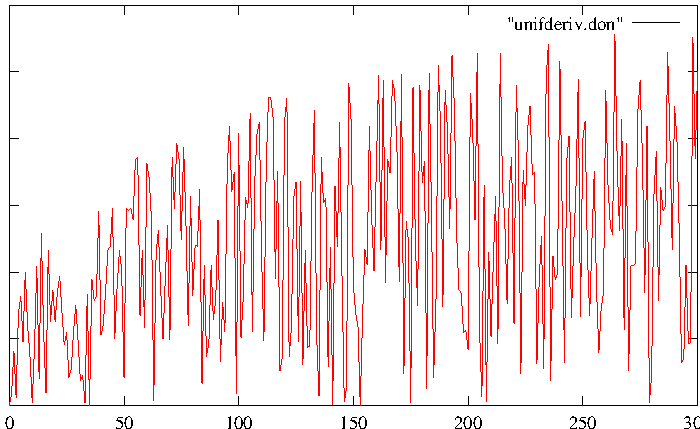
\includegraphics[width=5.5cm]{CE-unifderiv.pdf}
\end{center}
\pause
\begin{block}{Tendency analysis}
\alert{\bf non homogeneous experiment}

$\Rightarrow$ model the evolution of experiment

estimate and compensate tendency

\textcolor{blue}{\bf explain why}
\end{block}
\end{frame}
\begin{frame}{Control of experiments (2)}
\begin{center}
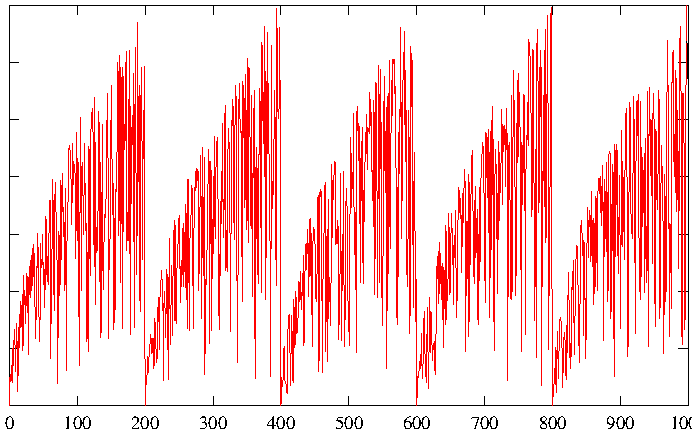
\includegraphics[width=5.5cm]{CE-periode.pdf}
\end{center}
\pause
\begin{block}{Periodicity analysis}
\alert{\bf periodic evolution of the experimental environment ?}

$\Rightarrow$ model the evolution of experiment

Fourier analysis of the sample

Integration on time (sliding window analysis) Danger : size of the window

Wavelet analysis

\textcolor{blue}{\bf explain why}
\end{block}
\end{frame}
\begin{frame}{Control of experiments (3)}
\begin{center}
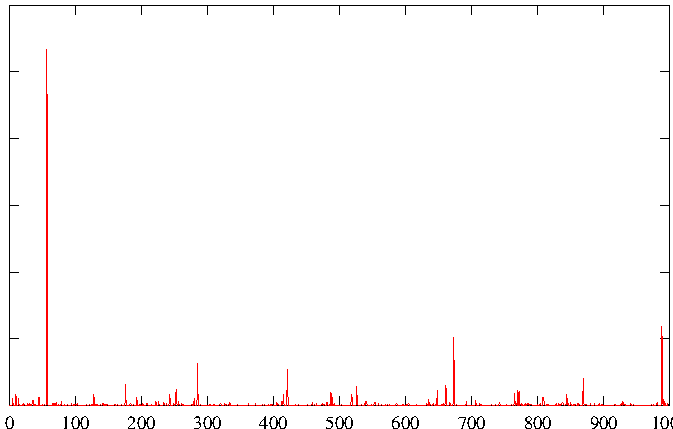
\includegraphics[width=5.5cm]{CE-cauchy1.pdf}
\end{center}
\pause
\begin{block}{Non significant values}
\alert{\bf  extraordinary behaviour of experimental environment}

rare events with different orders of magnitude

$\Rightarrow$ threshold by value \\
Danger : choice of the threshold : indicate the rejection rate

$\Rightarrow$ threshold by quantile \\
Danger : choice of the percentage : indicate the rejection value

\textcolor{blue}{\bf explain why}
\end{block}
\end{frame}

\begin{frame}{Control of experiments (4)}
Threshold value : 10
\begin{center}
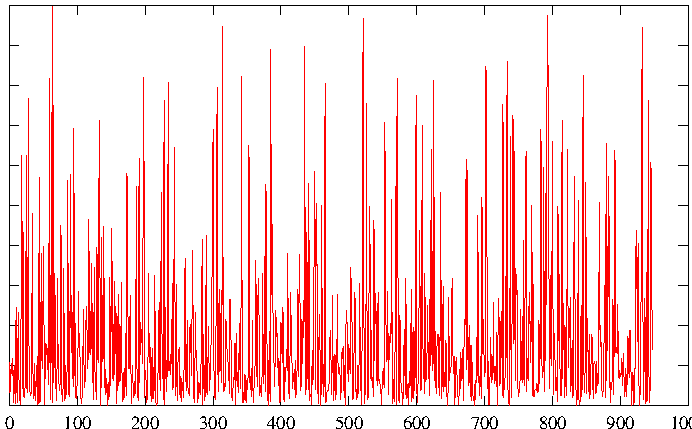
\includegraphics[width=5cm]{CE-cauchy-seuil10.pdf}
\end{center}
Threshold percentage  : 1\%
\begin{center}
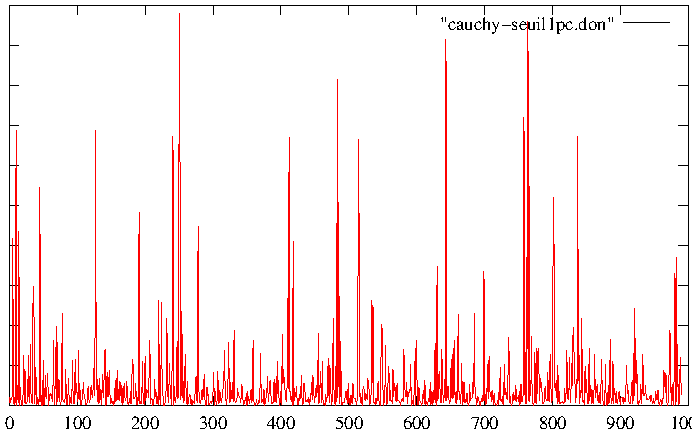
\includegraphics[width=5cm]{CE-cauchy-seuil1pc.pdf}
\end{center}

\end{frame}
\begin{frame}{Control of experiments (5)}
\begin{center}
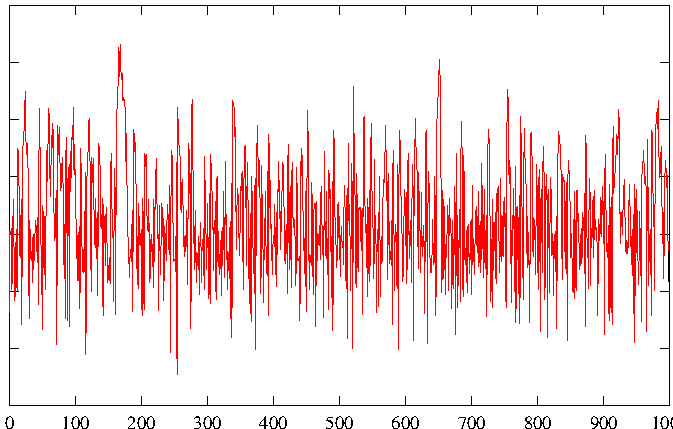
\includegraphics[width=5.5cm]{CE-deptempo.pdf}
\end{center}
\pause
\begin{block}{}
\alert{\bf  looks like correct experiments}

Statistically independent

Statistically homogeneous
\end{block}
\end{frame}

\begin{frame}{Control of experiments (5bis)}
Zooming
\begin{center}
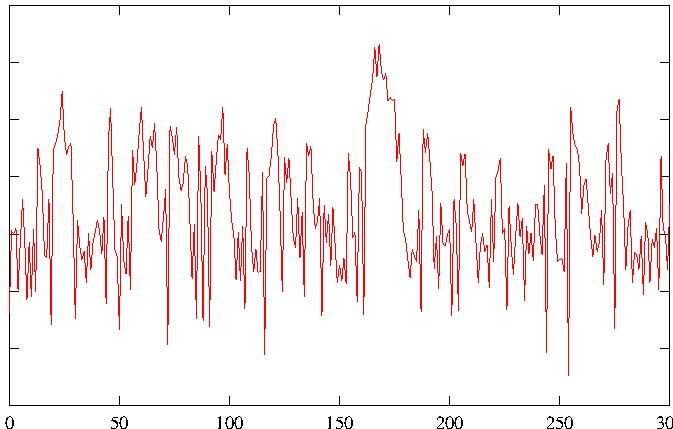
\includegraphics[width=5.5cm]{CE-deptempo-zoom.pdf}
\end{center}
\pause
\begin{block}{Autocorrelation}
Danger time correlation among samples

\alert{\bf  experiments impact on experiments}

$\Rightarrow$ stationarity analysis

autocorrelation estimation (ARMA)
\end{block}
\end{frame}
\section[{\scshape Sample Analysis}]{{\scshape Sample Analysis}}

\section{Analysis of Experiments}
\begin{frame}{Experimental results}
\begin{itemize}
\item Deterministic (controlled error non significant (white noise))
\item Statistic (the system is non deterministic)
\end{itemize}
\begin{block}{Sample analysis}
\begin{itemize}
\item Identification of the response set
\item Structure of the response set (measure)
\end{itemize}

\end{block}
\end{frame}

\begin{frame}{Distribution  analysis}
Summarize data in a {\bf histogram}
\begin{center}
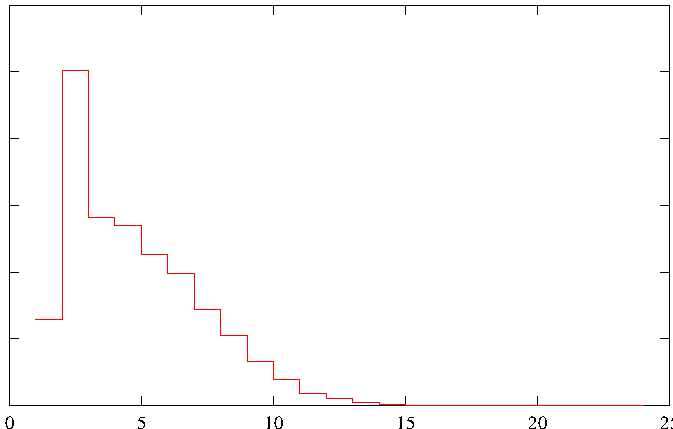
\includegraphics[width=4.6cm]{histogramme.pdf}
\end{center}
\begin{block}{Shape analysis}
\begin{itemize}
\item unimodal / multimodal
\item variability
\item symmetric / dissymmetric (skewness)
\item flatness (kurtosis)
\end{itemize}
\alert{\bf $\Longrightarrow$ Central tendency analysis} 

\alert{\bf $\Longrightarrow$ Variability analysis around the central tendency} 

\end{block}
\end{frame}
\section[{\scshape Central Tendency}]{{\scshape Central Tendency}}
\begin{frame}{Mode value}
{\bf histogram}
\begin{center}
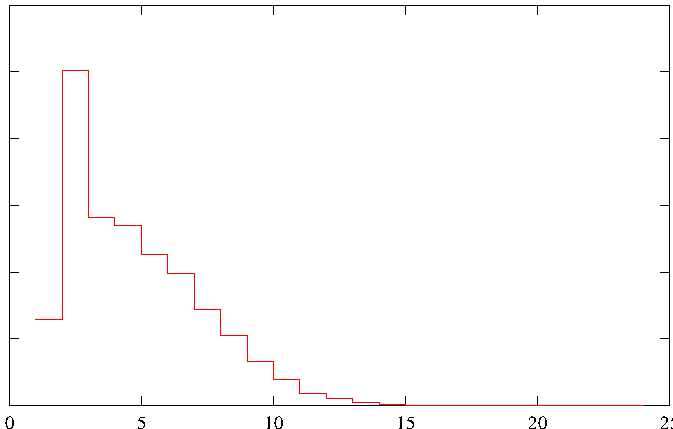
\includegraphics[width=4.6cm]{histogramme.pdf}
\end{center}
\begin{block}{Mode}
\begin{itemize}
\item  {\textcolor{Green4}{\bf Categorical data}}
\item Most frequent value
\item highly unstable value
\item for continuous value distribution depends on the histogram step
\item interpretation depends on the flatness of the histogram
\end{itemize}
\alert{\bf $\Longrightarrow$ Use it carefully} 

\alert{\bf $\Longrightarrow$ Predictor function} 

\end{block}
\end{frame}
\begin{frame}{Median value}
{\bf histogram}
\begin{center}
%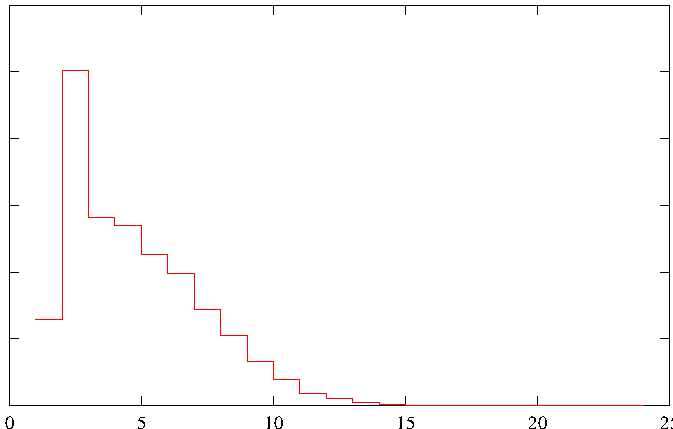
\includegraphics[width=4.6cm]{histogramme.pdf}
\end{center}
\begin{block}{Median}
\begin{itemize}
\item {\textcolor{Green4}{\bf Ordered data}}
\item Split the sample in two equal parts 
\[
\sum_{i\leq Median}f_i \leq \frac 1 2 \leq \sum_{i\leq Median+1}f_i .\]
\item more stable value
\item does not depends on the histogram step 
\item difficult to combine (two samples)
\end{itemize}


\alert{\bf $\Longrightarrow$ Randomized algorithms} 

\end{block}
\end{frame}
\begin{frame}{Mean value}
{\bf histogram}
\begin{center}
%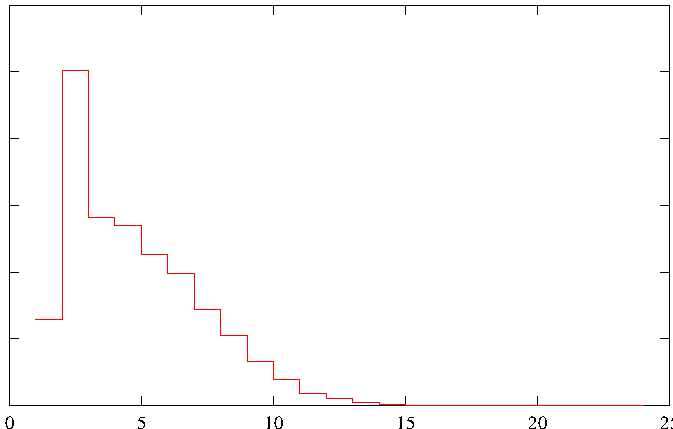
\includegraphics[width=4.6cm]{histogramme.pdf}
\end{center}
\begin{block}{Mean}
\begin{itemize}
\item {\textcolor{Green4}{\bf Vector space}}
\item Average of values 
\[
Mean = \frac 1 {Sample\_Size}\sum x_i = \sum_{x}x.f_x .\]
\item stable value 
\item does not depends on the histogram step 
\item easy to combine (two samples $\Rightarrow$ weighted mean)
\end{itemize}


\alert{\bf $\Longrightarrow$ Additive problems (cost, durations, length,...)} 

\end{block}
\end{frame}
\begin{frame}{Central tendency}
{\bf histogram}
\begin{center}
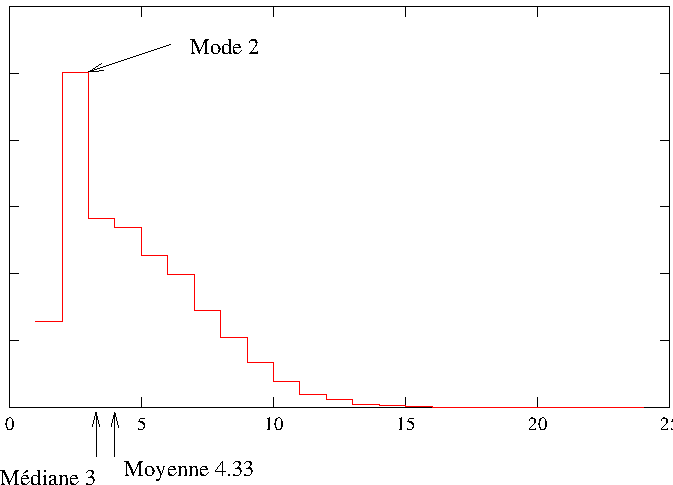
\includegraphics[width=4.6cm]{histogramme2.pdf}
\end{center}
\begin{block}{Complementarity}
\begin{itemize}
\item Valid if the sample is "Well-formed"
\item {\textcolor{Green4}{\bf Semantic of the observation}}
\item Goal of analysis 
\end{itemize}

\alert{\bf $\Longrightarrow$ Additive problems (cost, durations, length,...)} 

\end{block}
\end{frame}
\begin{frame}{Central tendency (2)}
\begin{block}{Summary of Means}
\begin{itemize}
\item Avoid means if possible\\
Loses information
\item  \textcolor{blue}{Arithmetic mean}\\
 When sum of raw values has physical meaning\\
Use for summarizing times (not rates)
\item \textcolor{blue}{Harmonic mean}\\
Use for summarizing rates (not times)
\item \textcolor{blue}{Geometric mean}\\
 Not useful when time is best measure of perf\\
 Useful when multiplicative effects are in play
\end{itemize}
\end{block}
\end{frame}
\section[{\scshape Variability}]{{\scshape Variability}}

\begin{frame}{Variability}
\begin{block}{Categorical data (finite set)}
$f_i$ : empirical frequency of element $i$

Empirical entropy
\[
H(f)=\sum_i f_i \log f_i.\]
Measure the empirical distance with the uniform distribution
\begin{itemize}
\item $H(f)\geq 0$
\item $H(f)=0$ iff the observations are reduced to a unique value
\item $H(f)$ is maximal for the uniform distribution
\end{itemize} 
\end{block}
\end{frame}
\begin{frame}{Variability (2)}
\begin{block}{Ordered data }

Quantiles : quartiles, deciles, etc

Sort the sample : 
\[
(x_1,x_2,\cdots ,x_n)\longrightarrow  (x_{(1)},x_{(2)},\cdots ,x_{(n)});\]
\[
Q_1=x_{(n/4)};\; Q_2=x_{(n/2)}=Median;\; Q_3=x_{(3n/4)}.\]

For deciles
\[
d_i = argmax_i \{\sum_{j\leq i}f_j \leq \frac i {10}\}.\]
Utilization as quantile/quantile plots to compare distributions
\end{block}
\end{frame}
\begin{frame}{Variability (3)}
\begin{block}{ Vectorial data }

Quadratic error for the mean 
\[
Var(X)=\frac 1 n \sum_1^n (x_i-\bar{x}_n)^2.\]
{\bf Properties:}
\begin{eqnarray*}
Var(X) & \geq & 0;\\
Var(X)&=&\overline{x^2}-(\bar{x})^2, \;\;\mbox{o\`u} \;\;\overline{x^2}=\frac 1 n \sum_{i=1}^n x_i^2.\;\\
Var(X+cste)&=&Var(X);\\
Var(\lambda X)&=&\lambda^2 Var(X).
\end{eqnarray*}

\end{block}
\end{frame}

\end{document}

\begin{frame}{Data Production}
\begin{alertblock}{Global Process}
\centerline{\alert{\textbf{\large Question $\Longrightarrow$ Experiment, Survey $\Longrightarrow$  Decision}}}

\vspace{0.5cm}

\centerline{\alert{\textbf{\large Decision = Risk }}}

\end{alertblock}
\pause
\begin{alertblock}{Quality of Data }
Specification of the Data
\begin{itemize}
\item Error model for the values
\item Experimental/Survey bias  
\item Analysis limitations
\end{itemize}
\end{alertblock}
\centerline{\colorbox{yellow!85}{\textcolor{black}{\textbf{\large Evaluate the Quality of the Decision}}}}
\end{frame}

\section[{\scshape Set of Variables}]{{\scshape Set of Variables} }

\begin{frame}{Criteria for the Quality of Data (from EuroStat)}
\begin{alertblock}{Relevance}
%Relevance is the degree to which statistics meet current and potential user needs. It refers to
%whether all statistics that are needed are produced and the extent to which concepts (definitions,
%classifications etc.) reflect user needs.
%The relevance of statistical information reflects the degree to which it meets the real needs of clients. It is concerned with whether the available information sheds light on the issues of most importance to users. Assessing relevance is a subjective matter dependent upon the varying needs of users. The NSO’s challenge is to weigh and balance the conflicting needs of different users to produce a program that goes as far as possible in satisfying the most important needs and users within given resource constraints
\begin{itemize}
\item degree to which statistics meet current and potential  needs
\item could extend to varying needs
\end{itemize}
\end{alertblock}
\pause
\begin{alertblock}{Accuracy}
%Accuracy in the general statistical sense denotes the closeness of computations or estimates
%to the (unknown) exact or true values. Statistics are never identical with the true values because
%of variability (the statistics change from implementation to implementation of the survey
%due to random effects) and bias (the average of the estimates from each implementation
%is not equal to the true value due to systematic effects). A basic distinction is between sampling
%and non-sampling errors, which are both subject to variability as well as bias.
%The accuracy of statistical information is the degree to which the information correctly describes the phenomena it was designed to measure. It is usually characterized in terms of error in statistical estimates and is traditionally decomposed into bias (systematic error) and variance (random error) components. It may also be described in terms of the major sources of error that potentially cause inaccuracy (e.g., coverage, sampling, non-response, response).
\begin{itemize}
\item Closeness of computations or estimates to the (unknown) exact or true values
\item Variability (random error) and bias (systematic error)
\item Sources of errors (experimental, coverage sampling...)
\end{itemize}
\end{alertblock}
\pause
\begin{alertblock}{Timeliness}
%Timeliness of information reflects the length of time between its availability and the event or
%phenomenon it describes. Punctuality refers to the time lag between the release date of data and the target date when it should have been delivered, for instance, with reference to dates
%announced in some official release calendar, laid down by regulations or previously agreed
%among partners.
%The timeliness of statistical information refers to the delay between the reference point (or the end of the reference period) to which the information pertains, and the date on which the information becomes available. It is typically involved in a trade-off against accuracy. The timeliness of information will influence its relevance.
\begin{itemize}
\item delay between the reference point and the availability date
\item trade-off against accuracy, 
\end{itemize}
\end{alertblock}
%\vfill 
%
%\centerline{\colorbox{yellow!85}{\textcolor{black}{\textbf{\large Take time to build a serious metadata document}}}}

\end{frame}
\begin{frame}{Criteria for the Quality of Data (from EuroStat)}
\begin{alertblock}{Comparability}
%Comparability aims at measuring the impact of differences in applied statistical concepts and
%measurement tools/procedures when statistics are compared between geographical areas,
%non-geographical domains, or over time. It is the extent to which differences between statistics
%are attributed to differences between the true values of the statistical characteristic.
%There are three main approaches under which comparability of statistics is normally
%addressed: comparability over time, between geographical areas, and between domains.
\begin{itemize}
\item measuring the impact of differences in applied statistical concepts and
measurement tools/procedures when statistics are compared between geographical areas,
non-geographical domains, or over time
\end{itemize}
\end{alertblock}
\pause
\begin{alertblock}{Coherence}
%Coherence of statistics is their adequacy to be reliably combined in different ways and for
%various uses. When originating from different sources, and in particular from statistical surveys
%of different nature and/or frequencies, statistics may not be completely coherent in the
%sense that they may be based on different approaches, classifications and methodological
%standards.
\begin{itemize}
\item adequacy to be reliably combined in different ways 
\item compatibility of measures 
\end{itemize}
\end{alertblock}
\pause
\begin{alertblock}{Accessibility}
%Accessibility refers to the physical conditions under which users can obtain data: where to
%go, how to order, delivery time, clear pricing policy, convenient marketing conditions (copyright,
%etc.), availability of micro or macro data, various formats (paper, files, CD-ROM, Internet
%etc.) etc.
%
%Clarity refers to the data’s information environment whether data are accompanied with
%appropriate documentation and metadata, illustrations such as graphs and maps, whether
%information on their quality is also available (including limitation in use etc.) and the extent to
%which additional assistance is provided by the NSI.
%The accessibility of statistical information refers to the ease with which it can be obtained from the NSO. This includes the ease with which the existence of information can be ascertained, as well as the suitability of the form or medium through which the information can be accessed. The cost of the information may also be an aspect of accessibility for some users.
\begin{itemize}
\item Accessibility refers to the physical conditions under which users can obtain data
\item Clarity refers to the data’s information environment
\end{itemize}
\end{alertblock}

\vfill

Extracted from \textit{Handbook on Data Quality
Assessment Methods and Tools} EuroStat Report (2013)
\end{frame}
\begin{frame}{Other Criteria for the Quality of Data \\(from Berti-Equille (2007))}
\begin{alertblock}{Interpretability}
%The interpretability of statistical information reflects the availability of the supplementary information and metadata necessary to interpret and utilize it appropriately. This information normally covers the underlying concepts, variables and classifications used, the methodology of collection, and indications of the accuracy of the statistical information.
\begin{itemize}
\item availability of the supplementary information and metadata
\item covers the underlying concepts
\end{itemize}
\end{alertblock}
\begin{alertblock}{Unicity}
%Unicité : garantie qu’une entité du monde réel est représentée par un seul et unique objet, il s’agit de contrôler la présence des doublons.
\begin{itemize}
\item one physical observation is represented by a unique object in the Dataset
\item no duplicates
\end{itemize}
\end{alertblock}
\begin{alertblock}{Conformity to Norm}
%Conformité à une norme : respect d’une norme standardisée ou d’une convention de nommage (p.ex., la profession de la personne est codée selon la norme INSEE : PCS en 8 catégories).
\begin{itemize}
\item use the standardized encoding (reals, strings, statistical variables)
\end{itemize}
\end{alertblock}
\begin{alertblock}{Consistency}
%Consistance : Quand une entité est recopiée, il y a consistance si on retrouve les mêmes valeurs d’attributs dans toutes les bases. 
\begin{itemize}
\item duplicated informations have the same value 
\end{itemize}
\end{alertblock}
\end{frame}

\section[{\scshape Missing Values}]{{\scshape Missing Values} }
\begin{frame}{Pre-processing of Data}
\centerline{\colorbox{yellow!85}{\textcolor{black}{\textbf{\large Before any analysis : check the Data}}}}
\begin{alertblock}{Question on the Quality}
\begin{itemize}
\item Are there missing values ?  almost yes
\item How many sampling are missing ?
\item Is there a bias for missing data or randomly spread ?
\item Is the bias in the dataset sufficiently important to modify the analysis (estimators, tests,...) ?
\end{itemize}
\centerline{\colorbox{yellow!85}{\textcolor{black}{\textbf{\large Give potential explanations}}}}
\end{alertblock}
\pause

\begin{alertblock}{Identification of Data Problems}
Model of the Dataset (types, semantic,...)
\begin{itemize}
\item Missing Data (none or partial  value)
\item Non relevant 
\item Duplicated
\end{itemize}
\centerline{\colorbox{yellow!85}{\textcolor{black}{\textbf{\large Give potential explanations}}}}
\end{alertblock}
\end{frame}
\begin{frame}{Pre-processing of Data (2)}
\begin{alertblock}{Distributions of Data Problems }
Analyse the position of missing values in the Dataset
\begin{itemize}
\item MCAR, Missing Completely at random (unpredictable missing)
\item MAR, Missing at random (predictable values : model)
\item MNAR, Non missing at random
\end{itemize}
\end{alertblock}
\pause

\begin{alertblock}{Processing Missing Data}
\begin{itemize}
\item Do nothing 
\item Remove samples with missing values
\item Weighted analysis 
\item Value imputation (central tendency, EM, regression, random hot deck, neighbouring,...)
\end{itemize}
\centerline{\colorbox{yellow!85}{\textcolor{black}{\textbf{\large Report the method that has been used}}}}

\end{alertblock}
\end{frame}
\end{document}
